
%version 2: \usepackage{hyperref}


%%%%%%%%%%%%%%%%%%%%%%%%%%%%%%%%%%%%%%%%%%%%%%%%%%%%%%%%%%%%%%%%%%%%%%%%
%Para las ecuaciones siempre es Ec.(n).
%Para las figuras siempre es Fig.n, incluso en el caption de la figura. Tambien las Tablas
%Para las referencias es [n]
%%%%%%%%%%%%%%%%%%%%%%%%%%%%%%%%%%%%%%%%%%%%%%%%%%%%%%%%%%%%%%%%%%%%%%%%

\documentclass[
reprint,
%notitlepage,
%superscriptaddress,
%groupedaddress,
%unsortedaddress,
%runinaddress,
%frontmatterverbose, 
%preprint,
%showpacs,preprintnumbers,
%nofootinbib,
%nobibnotes,
%bibnotes,
%11 pt,
amsmath,
amssymb,
aps,
pra,
%prb,
%rmp,
%tightenlines %esto hizo el milagro de sacar los espacios en blancos estocásticos (?)
%prstab,
%prstper,
%floatfix,\textbf{}
]{revtex4-1} %Instalar primero para usarlo. Paquete malo.

%\documentclass[onecolumn, aps, amsmath,amssymb ]{article}
\usepackage{lipsum}  
\usepackage{graphicx}% Include figure files
\usepackage{subfig}
\usepackage{braket}
\usepackage{comment} %comment large chunks of text
\usepackage{dcolumn}% Align table columns on decimal point
\usepackage{bm}% bold math
%\usepackage{hyperref}% add hypertext capabilities
\usepackage[mathlines]{lineno}% Enable numbering of text and display math
%\linenumbers\relax % Commence numbering lines
\usepackage{mathtools} %% Para el supraíndice

\usepackage[nice]{nicefrac}

%%%%%%%El Señor Español%%%%%%%%%%%%%%%%%%%%%%%%%%%
\usepackage[utf8]{inputenc} %acento
\usepackage[
spanish, %El lenguaje.
es-tabla, %La tabla y no cuadro.
activeacute, %El acento.
es-nodecimaldot %Punto y no coma con separador de números
]{babel}
\usepackage{microtype} %para hacerlo más bonito :33 como vos (?) 
%%%%%%%%%%%%%%%%%%%%%%%%%%%%%%%%%%%%%%%%%%%%%%%%%%%
%%%%%%%%% Para que las imágenes se queden dónde las quiero (?
\usepackage{float}
%%%%%%%%%%

\usepackage{hyperref} % Para usar \url

%%%%%%%%Cambia a Fig de Figure%%%%%%%%%%
\makeatletter
\renewcommand{\fnum@figure}{Fig. \thefigure} 
\makeatother
%%%%%%%%%%%%%%%%%%%%%%%%%%%%%%%%%%%%%%%%
\raggedbottom


\begin{document}
%%%%%%%%%%%%%%%%%%%%%%%%%%%%%%%%%%Título%%%%%%%%%%%%%%%%%%%%%%%%%%%%%%%%%%%%%%
%%%%%%%%%%%%%%%%%%%%%%%%%%%%%%%%%%%%%%%%%%%%%%%%%%%%%%%%%%%%%%%%%%%%%%%%%%%%%%

\title{Modulación del clima para el archivo de todos los disparos en el rango 2014-2020}
\author{Evelyn~G.~Coronel}

\affiliation{
Tesis de Maestría en Ciencias Físicas\\ Instituto Balseiro\\}

\date[]{\lowercase{\today}} %%lw para lw, [] sin date

%\begin{abstract}

%\end{abstract} 
\maketitle
%%%%%%%%%%%%%%%%%%%%%%%%%%%%%%%%%%%%%%%%%%%%%%%%%%%%%%%%%%%%%%%%%%%%%%%%%%%%%%%%%%%

Ahora tenemos el archivo del clima hasta el 16 de abril del 2020.

¿Qué estaba pasando? Cuando hacía la clasificación de los datos a utilizar para calcular los datos del clima, estaba considerando solo los 6T5. Ese filtro, en el bin de 1 EeV - 2 EeV, era para calcular la anisotropía solamente. En los parámetros del clima, nos sirven los 5T5. \textbf{En cambio en la anisotropía, solo consideramos los 6T5}.


Otra cosa que hablamos durante la presentación del beamer, fue la sectancia (sic, Allekotte). En el bin 1 EeV - 2 EeV, los eventos están bien reconstruidos \footnote{¿según que parámetro está bien reconstruído? ¿$\chi^2$? Entiendo que la lluvia los eventos verticales de baja energía tienen una componente e.m. pequeña por el damping de la atmósfera cuando están muy inclinadas.} para sectancia menor a $60^o$.


Ahora, ya al principio de todo el proceso de análisis del clima y de anisotropía, al extraer los datos de los archivos del Herald, tiene en cuenta \textbf{solamente} los eventos de $\theta < 60^o$ \footnote{el archivo que bajo de \url{http://ipnwww.in2p3.fr/~augers/AugerProtected/herald.php} }. Esto sucede en el archivo $\text{energy\_filter\_AllTriggers.sh}$, que calcula los eventos para el análisis de anisotropía en el bin 1 EeV - 2 EeV, y para $\text{energy\_filter\_AllTriggers.sh}$, que calcula los eventos con energía mayor a 1 Eev para obtener los parámetros del clima. El parámetro $ib$ para los eventos es aplicado para los \textbf{eventos del herald } en los mismos código. 

El parámetro de $ib$ de los \textbf{datos del clima} es irrelevante durante el proceso de filtrar eventos. Entra en juego cuando hago el análisis del clima, donde desecho los eventos que fueron recabados durante \emph{bad weather} \textbf{y} no fueron filtrados ya antes.


\section{Pesos de los hexágonos}

\begin{figure}[H]
	\centering
	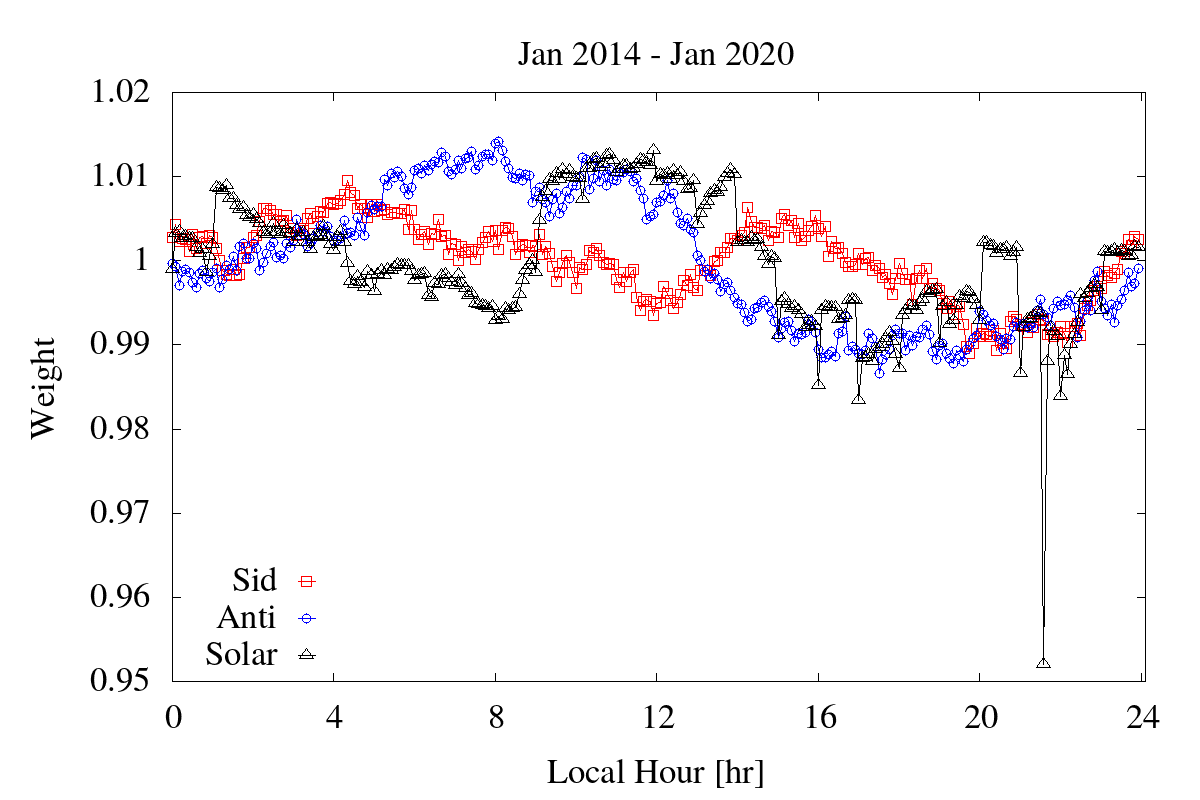
\includegraphics[width=0.5\textwidth]{weigth2014-2020_jan.png}
\end{figure}

\section{Anisotropía}

En el rango $1372680308$ \footnote{Mon, 1 July 2013 12:05:08 GMT} y $1388577600$ \footnote{Thur, 1 January 2014 12:00:00 GMT}, la tasa de eventos del archivo $\text{All Triggers}$, tenía una tasa de eventos por debajo de los normal. Por esto, se utiliza los eventos a partir del  1388577600. La tasa de eventos que se utiliza se puede ver  a continuación:

\begin{figure}[H]
	\centering
	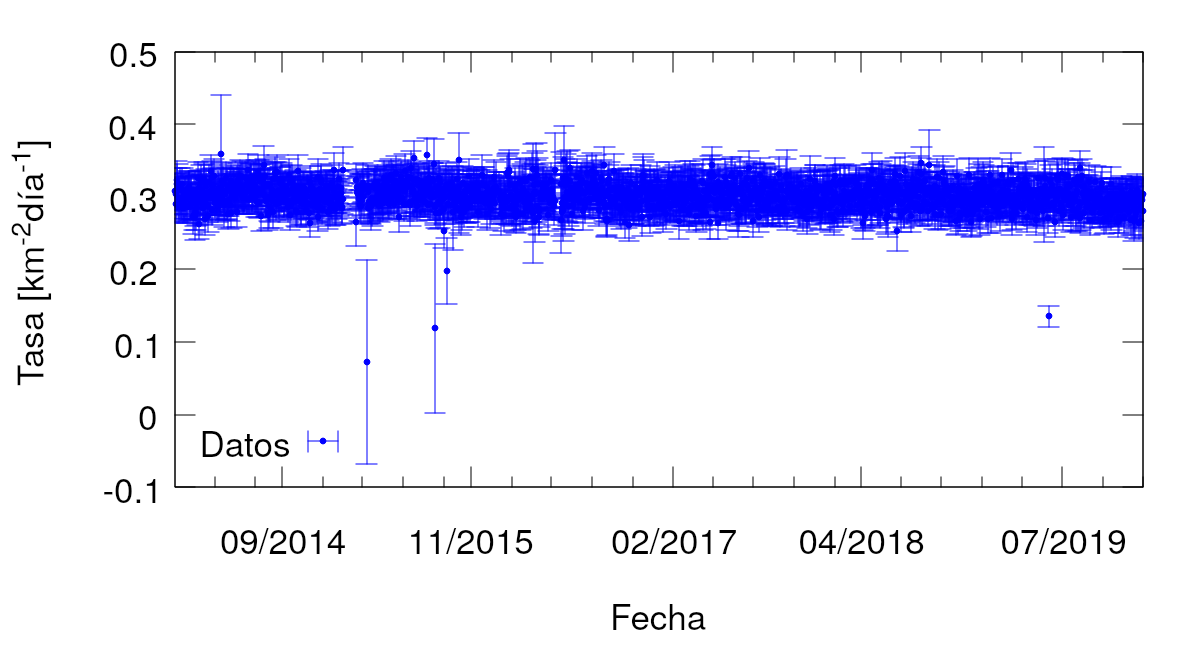
\includegraphics[width=0.5\textwidth]{rate_total.png}
\end{figure}


\subsection{Filtro de datos detallado}
Esta sección muestra la anisotropía en el 1 EeV - 2 EeV, tomando los siguientes filtros de eventos:

\begin{enumerate}
	\item Energía entre  [1 EeV , 2 EeV)
	\item Rango de tiempo:
	\begin{itemize}
		\item[-] Inicial:1388577600 \\ (Thursday, 1 January 2014 12:00:00 GMT)
		\item[-] Final: 1577880000  \\ (Thursday, 1 January 2020 12:00:00 GMT)
	\end{itemize}
	\item Sectancia:  $\theta < 60^o$
	\item $iw<4$ (weather quality flag)
	\item 6T5
	\item $ib=1$ Bad period flag
\end{enumerate}


Con estos filtros se tienen $1\,092\,753$ eventos

\subsection{Análisis en frecuencia}

\begin{figure}[H]
	\centering
	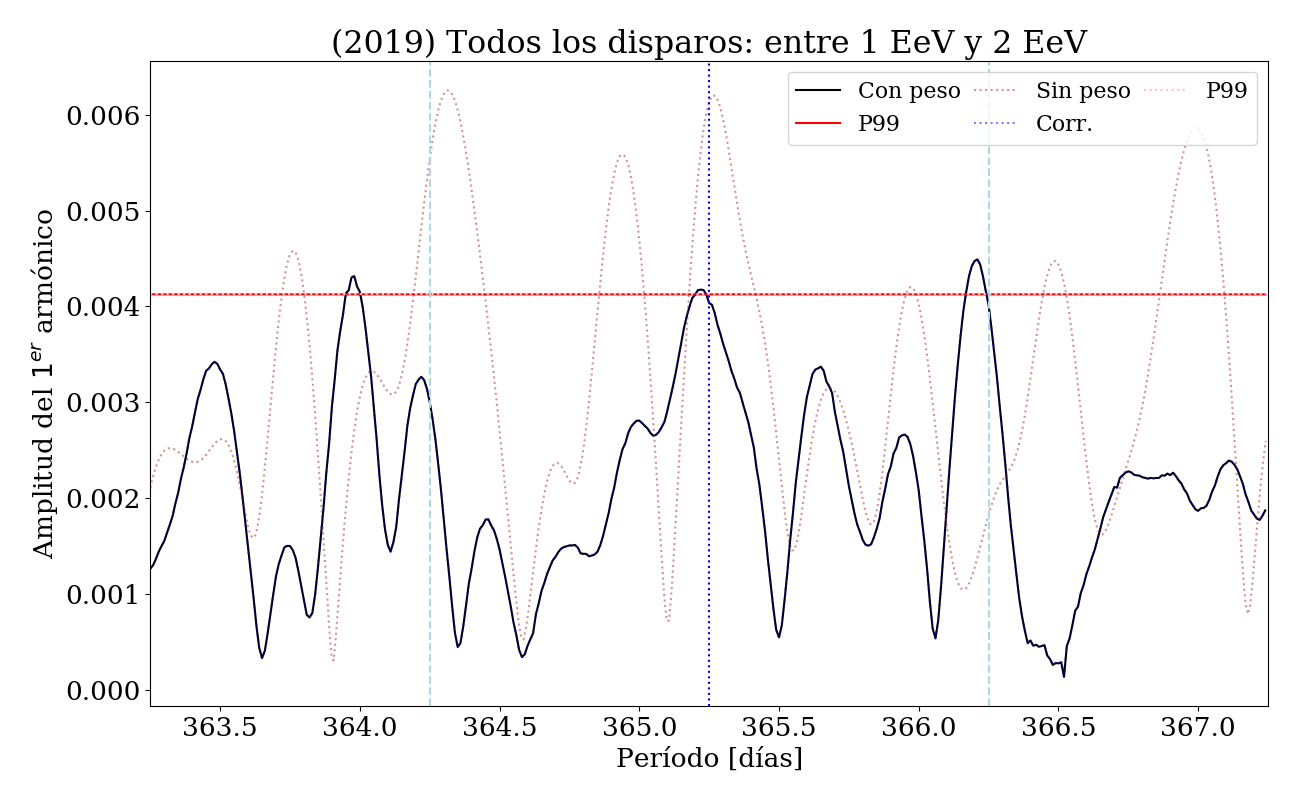
\includegraphics[width=0.5\textwidth]{2019_AllTriggers_1_2_EeV_con_vs_sin_peso.png}
	\caption{Análisis en frecuencia en ascensión recta en rango 1 EeV - 2 EeV}
	\label{fig:consin}
\end{figure}


\section{Corrección del clima}

\begin{figure}[H]
	\centering
	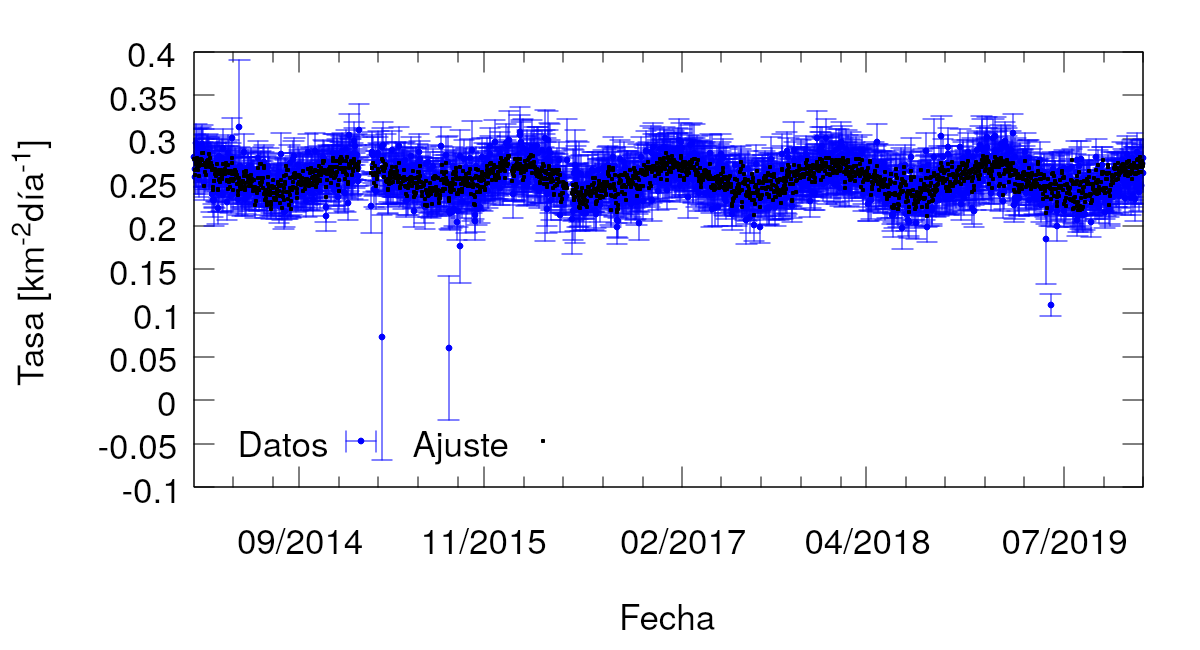
\includegraphics[width=0.5\textwidth]{rate_Ajuste.png}
\end{figure}



\begin{figure}[H]
	\centering
	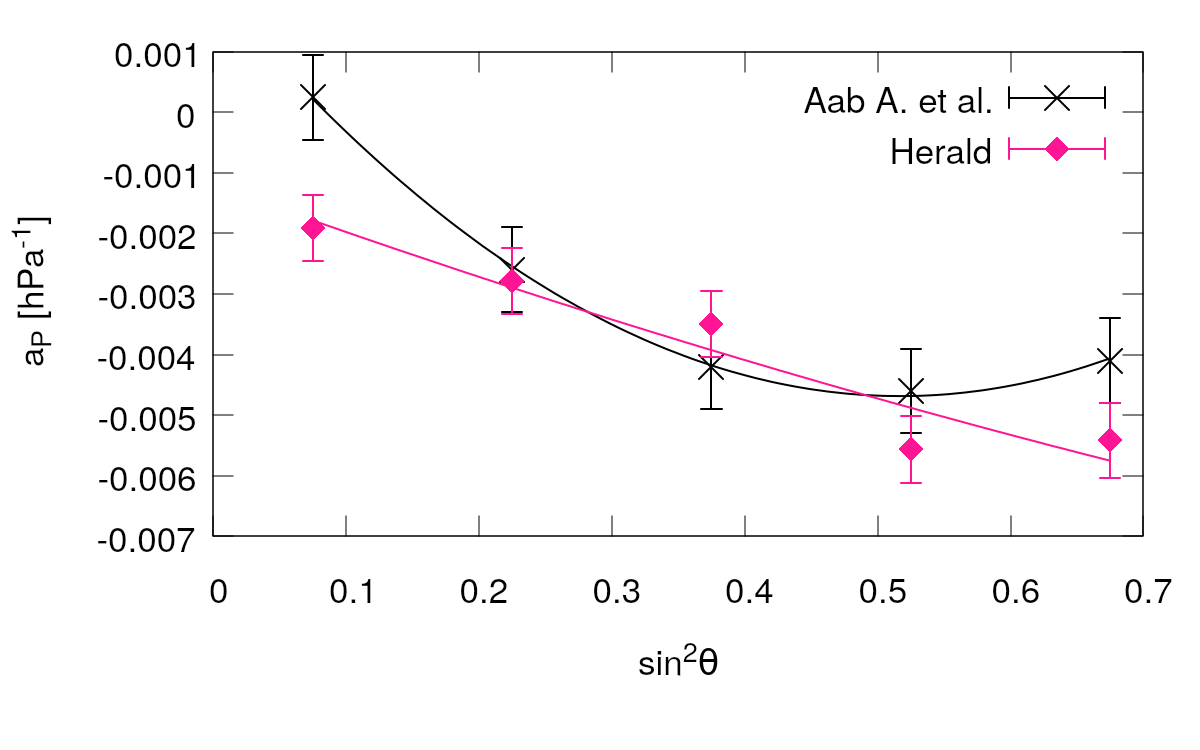
\includegraphics[width=0.5\textwidth]{ap.png}
\end{figure}

\begin{figure}[H]
	\centering
	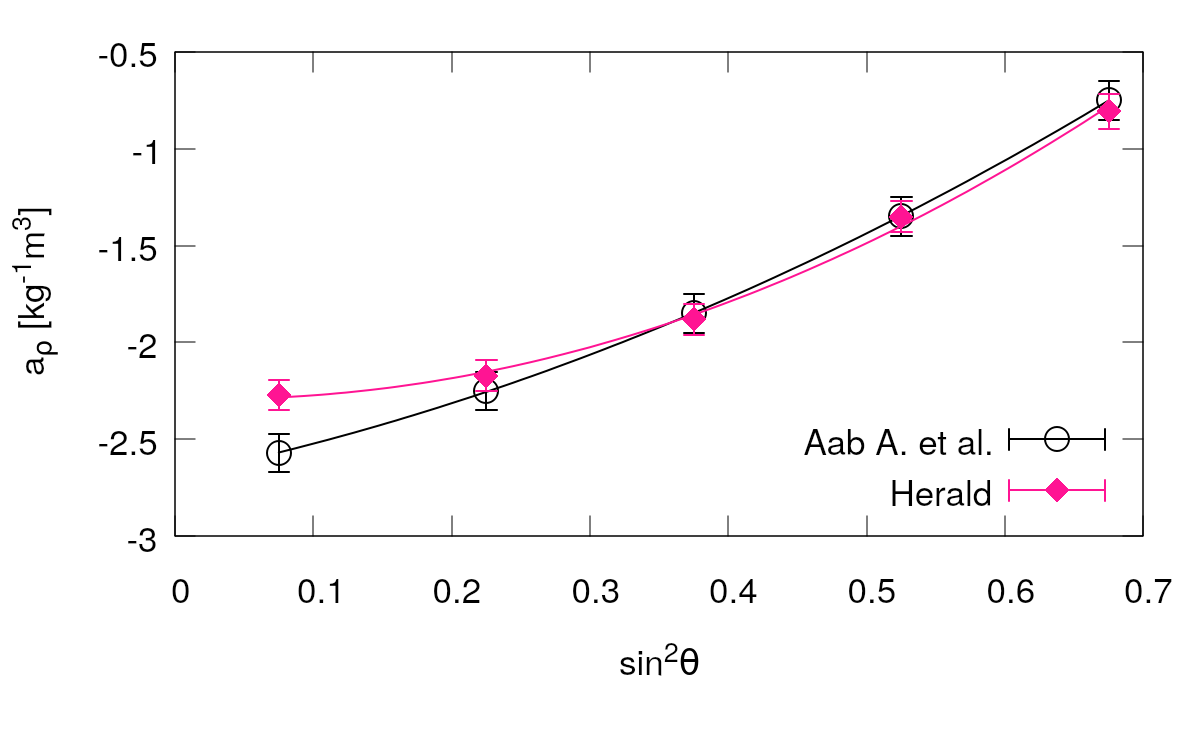
\includegraphics[width=0.5\textwidth]{arho.png}
\end{figure}

\begin{figure}[H]
	\centering
	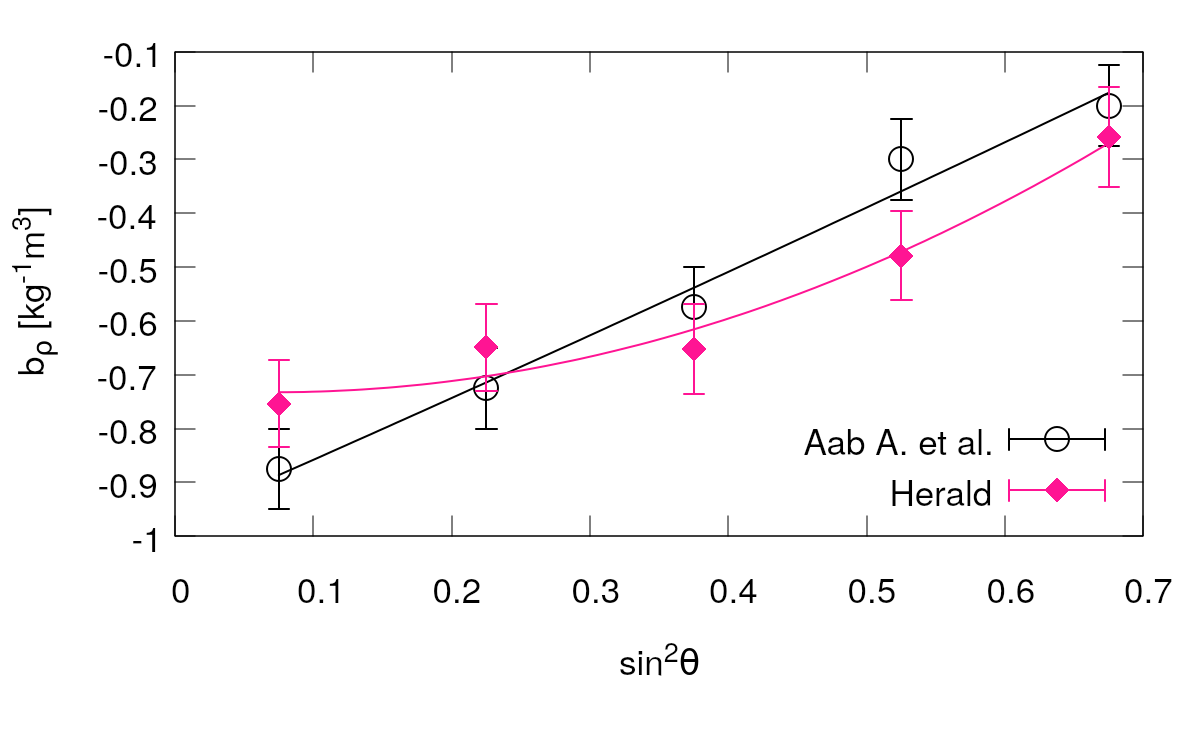
\includegraphics[width=0.5\textwidth]{brho.png}
\end{figure}


\end{document}

